\documentclass[onecolumn]{jmlr}

\usepackage{booktabs}
\usepackage{graphicx}
\usepackage{array}
\usepackage{amsmath}
\usepackage{url}

\title{Detecting AI-Generated Hotel Reviews with Classical Text Classifiers}
\author{%
\vspace{\baselineskip}%
\begin{tabular*}{\textwidth}{@{}l@{\extracolsep{\fill}}r@{}}
Jiacheng Cai & \texttt{j.cai5@students.uu.nl} \\
Rongjian Gao & \texttt{r.gao2@students.uu.nl} \\
Yanpeng Wang & \texttt{y.wang36@students.uu.nl}
\end{tabular*}}
\date{October 2026}

\begin{document}

\maketitle

\begin{abstract}
Online review platforms increasingly contain text generated by large language models, which makes authorship harder to assess from surface fluency alone. This study compares five classical text classifiers on a balanced English-language corpus of 1,000 human-written hotel reviews and 1,000 reviews generated by GPT-4. Reviews were represented as unigram count vectors after a small set of preprocessing decisions chosen on the training data. Multinomial naive Bayes, Lasso logistic regression, a classification tree, a random forest, and gradient boosting were tuned with five-fold cross-validation on 1,500 reviews and evaluated once on a held-out test set of 500 reviews. Random forest obtained the highest test accuracy, 0.934, followed by gradient boosting at 0.928 and Lasso logistic regression at 0.908, while multinomial naive Bayes and the single tree reached 0.888 and 0.816. McNemar tests found no significant difference between the two linear classifiers at the 0.01 level. Both tree ensembles performed significantly better than the single tree. Random forest accuracy was slightly higher for negative than for positive reviews (0.944 versus 0.924), but a Fisher exact test did not support a difference between the two sentiment groups. The most predictive terms suggest that the classifiers use a mixture of evaluative vocabulary, narrative wording, and frequent function words. These patterns are useful for interpretation, although several are also reminders that source-specific artifacts can contribute to measured performance.
\end{abstract}

\section{Introduction}

Consumers often rely on online reviews when choosing hotels and other services. The same platforms are vulnerable to deceptive reviews, and recent language models can produce fluent text with few obvious grammatical problems. This changes the detection problem. A classifier can no longer rely on poor writing quality as a general marker of deception; it must identify subtler differences in vocabulary and style.

We study English hotel reviews from the MAiDE-up corpus introduced by Ignat et al.\ \cite{ignat2025}. The task is binary classification: label 1 denotes a review generated by GPT-4, and label 0 denotes a human review collected from Booking.com. Our experiments address four questions. First, we compare multinomial naive Bayes, a generative linear model, with Lasso logistic regression, a discriminative linear model. Second, we test whether random forest and gradient boosting improve on a single classification tree. Third, we examine whether the selected random forest performs differently on positive and negative reviews. Finally, we inspect the most influential terms in each model and consider what they reveal about the classification task.

The study uses deliberately conventional methods. Bag-of-words features and classical classifiers are easier to reproduce and inspect than a large pretrained language model. They also make it possible to connect predictive performance to individual terms. This interpretability comes with limits: word counts discard context, and an important term is not necessarily a general linguistic marker of AI authorship.

\section{Data}

The corpus contains 2,000 English reviews: 1,000 human-written reviews and 1,000 GPT-4-generated reviews. Each class contains equal numbers of positive and negative reviews. The positive and negative parts supplied in the source data were concatenated to form the text used by the classifiers. Review score, city, and hotel name were retained as metadata but were not used as predictors.

We made one stratified random split at review level. The split used the joint combination of class label and sentiment, so each of the four strata contributed 375 reviews to the training set and 125 reviews to the test set. This produced 1,500 training reviews and 500 test reviews. The random seed was 42. The test set was kept separate during preprocessing decisions and hyperparameter selection.

\begin{table}[ht]
\centering
\caption{Distribution of reviews after the stratified split.}
\label{tab:split}
\begin{tabular}{lrrrrr}
\toprule
Split & Human neg. & Human pos. & AI neg. & AI pos. & Total \\
\midrule
Training & 375 & 375 & 375 & 375 & 1500 \\
Test     & 125 & 125 & 125 & 125 & 500 \\
\bottomrule
\end{tabular}
\end{table}

\section{Text preprocessing}

All text was converted to lowercase. Curly apostrophes were replaced with straight apostrophes, accents were removed, and the tokenizer retained alphabetic tokens and contractions while dropping numbers and punctuation. We kept stop words, did not apply stemming, and used unigram counts. Terms occurring in fewer than five training reviews were removed. The resulting training vocabulary contained 1,351 terms.

Before tuning any model, we compared seven preprocessing settings with five-fold cross-validation on the training set, using the same folds as in the later grid searches (Table~\ref{tab:prep} in Appendix~\ref{app:prep}). For this comparison naive Bayes used its default smoothing ($\alpha=1$) without feature selection, and the regularization strength of Lasso logistic regression was chosen by an inner five-fold cross-validation within each training fold. All settings reached between 0.885 and 0.909 accuracy, and most differences were smaller than one cross-validation standard deviation (about 0.01 for naive Bayes and 0.02 for logistic regression). No setting was clearly best, so the comparison mainly ruled out settings that were clearly worse, and the remaining choice was based on interpretability and vocabulary size. Removing stop words lowered the accuracy of both models slightly (from 0.901 to 0.897 for naive Bayes and from 0.899 to 0.893 for logistic regression). We kept them because function words such as \emph{I}, \emph{we}, and \emph{the} may capture writing style even when they carry little topic information. Stemming gave no consistent gain and made important terms harder to read. Raising the minimum document frequency from one to five reduced the vocabulary from 4,737 to 1,351 terms; naive Bayes accuracy rose by 0.7 percentage points and logistic regression accuracy fell by 1.0 point, both within the cross-validation noise. Adding bigrams nearly tripled the vocabulary and improved accuracy by at most 0.7 points.

The vectorizer was included inside every model pipeline. During cross-validation, each fold therefore learned its vocabulary from that fold's training portion. This prevents validation reviews from influencing feature construction.

\section{Models and experimental setup}

We trained five classifiers. Multinomial naive Bayes modeled word counts with conditional independence between terms. A chi-squared filter selected the top $k$ terms before fitting the classifier. Logistic regression used an L1 penalty, which shrinks many word coefficients to zero and provides an embedded form of feature selection. The single classification tree used cost-complexity pruning. Random forest averaged multiple trees trained with feature subsampling, while gradient boosting fitted shallow trees sequentially.

We used the same five stratified folds for all grid searches. The folds were stratified by the combination of class label and sentiment. Accuracy was the tuning criterion. After selecting the best hyperparameters, each model was refitted on all 1,500 training reviews. The held-out test set was then used to estimate the performance of the five selected models. Table~\ref{tab:grids} in Appendix~\ref{app:grids} lists the full grids, and Appendix~\ref{app:curves} shows the cross-validation accuracy for every grid point. All other parameters were left at their scikit-learn defaults, with the random seed fixed to 42.

Our first grids for random forest and gradient boosting selected values on the edge of the grid. We therefore extended those grids in the direction of the edge until cross-validation accuracy stopped improving. In the final grids, the selected maximum number of features, learning rate, tree depth, $k$, $C$, and \texttt{ccp\_alpha} all lie strictly inside the searched range. The selected numbers of trees and boosting stages are the largest values searched, but accuracy had levelled off. For random forest, more trees reduce variance without increasing model complexity, and accuracy with three features per split changed by only 0.2 percentage points between 300 and 1,000 trees. For gradient boosting, the number of stages interacts with the learning rate. At learning rate 0.3, accuracy peaked at 200 to 400 stages and then declined. At learning rate 0.1, it rose by only 0.3 points from 400 to 800 stages, which indicates that the selected setting is close to the plateau.

\begin{table}[ht]
\centering
\caption{Selected hyperparameters and five-fold cross-validation accuracy. The searched grids are listed in Table~\ref{tab:grids}.}
\label{tab:tuning}
\small
\begin{tabular}{p{2.4cm}p{7.0cm}r}
\toprule
Model & Selected setting & CV accuracy \\
\midrule
Naive Bayes & $k=750$, $\alpha=0.5$ & 0.903 \\
Lasso logistic regression & $C=1$; 203 of 1,351 coefficients non-zero & 0.915 \\
Classification tree & $\mathrm{ccp\_alpha}=0.002$; 53 leaves & 0.818 \\
Random forest & 1,000 trees; 3 features per split & 0.919 \\
Gradient boosting & 800 stages; learning rate 0.1; depth 2 & 0.923 \\
\bottomrule
\end{tabular}
\end{table}

We report accuracy, precision, recall, and the $F_1$ score. AI-generated reviews are treated as the positive class.

\subsection{Statistical tests}

To test whether two classifiers $A$ and $B$ differ in accuracy, we use McNemar's test on their predictions for the same 500 test reviews \citep{dietterich1998}. Each test review falls into one cell of a $2\times2$ table, according to whether $A$ classified it correctly and whether $B$ did. Reviews on which both classifiers are correct, or both are wrong, say nothing about which classifier is more accurate. The test therefore uses only the two discordant counts: $n_{01}$, the number of reviews misclassified by $A$ but not by $B$, and $n_{10}$, the number misclassified by $B$ but not by $A$. Under the null hypothesis that $A$ and $B$ have the same error rate, a discordant review is equally likely to fall in either cell. Conditional on $n=n_{01}+n_{10}$, the count $n_{01}$ then follows a binomial distribution with $n$ trials and success probability $1/2$. We use the exact two-sided $p$-value
\begin{equation*}
p = \min\Bigl(1,\; 2\sum_{i=0}^{m}\binom{n}{i}\,2^{-n}\Bigr), \qquad m=\min(n_{01},n_{10}),
\end{equation*}
rather than the $\chi^2$ approximation $(|n_{01}-n_{10}|-1)^2/(n_{01}+n_{10})$ described by \citet{dietterich1998}. The exact test does not require a large number of discordant reviews. The null hypothesis is rejected when $p<0.01$.

The comparison between positive and negative reviews for random forest is of a different kind. The two sentiment subsets contain different reviews, so their accuracies are independent proportions and McNemar's test does not apply. We arrange the random forest predictions in a $2\times2$ table of sentiment (positive, negative) by outcome (correct, incorrect) and apply Fisher's exact test. Under the null hypothesis that accuracy does not depend on sentiment, and conditional on the row and column totals, the number of correctly classified positive reviews follows a hypergeometric distribution. The two-sided $p$-value is the total probability of all tables with the same margins that are no more likely than the observed table. We again use $\alpha=0.01$.

\section{Results}

\subsection{Predictive performance}

Table~\ref{tab:test-results} reports performance on the 500 held-out reviews. Random forest reached the highest accuracy, 0.934, and the highest precision, 0.966. Gradient boosting followed at 0.928 accuracy, with almost the same recall as random forest. Lasso logistic regression reached 0.908 accuracy. Naive Bayes had the highest recall, 0.940, but its lower precision shows that it classified more human reviews as AI generated. The single tree had the lowest values on all four measures.

\begin{table}[ht]
\centering
\caption{Performance on the held-out test set. AI-generated reviews are the positive class.}
\label{tab:test-results}
\begin{tabular}{lrrrr}
\toprule
Model & Accuracy & Precision & Recall & $F_1$ \\
\midrule
Naive Bayes & 0.888 & 0.851 & 0.940 & 0.894 \\
Lasso logistic regression & 0.908 & 0.918 & 0.896 & 0.907 \\
Classification tree & 0.816 & 0.838 & 0.784 & 0.810 \\
Random forest & 0.934 & 0.966 & 0.900 & 0.932 \\
Gradient boosting & 0.928 & 0.950 & 0.904 & 0.926 \\
\bottomrule
\end{tabular}
\end{table}

\subsection{Classifier comparisons}

Table~\ref{tab:mcnemar} gives the $2\times2$ table and the exact McNemar $p$-value for each comparison. Naive Bayes alone was correct on 31 reviews, while logistic regression alone was correct on 41. The resulting $p$-value of 0.289 is above 0.01, so the observed accuracy difference does not provide evidence that the two linear models have different error rates.

Both ensemble comparisons produced a different result. Random forest alone was correct on 70 reviews missed by the single tree, while the tree alone was correct on 11 reviews missed by the forest. Gradient boosting alone was correct on 68 reviews missed by the tree, compared with 12 in the other direction. Both differences were significant at the specified level.

\begin{table}[ht]
\centering
\caption{McNemar $2\times2$ tables on the 500 test reviews. Rows give the correctness of the first classifier, columns that of the second. The off-diagonal cells are the discordant counts used by the test.}
\label{tab:mcnemar}
\small
\begin{tabular}{@{}lrr@{}}
\toprule
 & \multicolumn{2}{c}{LR} \\
\cmidrule(l){2-3}
NB & Correct & Wrong \\
\midrule
Correct & 413 & 31 \\
Wrong & 41 & 15 \\
\midrule
\multicolumn{3}{@{}l}{exact $p=0.289$} \\
\bottomrule
\end{tabular}\hfill
\begin{tabular}{@{}lrr@{}}
\toprule
 & \multicolumn{2}{c}{RF} \\
\cmidrule(l){2-3}
Tree & Correct & Wrong \\
\midrule
Correct & 397 & 11 \\
Wrong & 70 & 22 \\
\midrule
\multicolumn{3}{@{}l}{exact $p=1.18\times10^{-11}$} \\
\bottomrule
\end{tabular}\hfill
\begin{tabular}{@{}lrr@{}}
\toprule
 & \multicolumn{2}{c}{GB} \\
\cmidrule(l){2-3}
Tree & Correct & Wrong \\
\midrule
Correct & 396 & 12 \\
Wrong & 68 & 24 \\
\midrule
\multicolumn{3}{@{}l}{exact $p=1.20\times10^{-10}$} \\
\bottomrule
\end{tabular}
\end{table}

\subsection{Random forest performance by sentiment}

Random forest classified 231 of 250 positive reviews and 236 of 250 negative reviews correctly. Accuracy and $F_1$ were slightly higher in the negative subset, mainly because recall for AI-generated negative reviews was 0.920 compared with 0.880 for positive reviews. Precision was almost the same in both groups.

\begin{table}[ht]
\centering
\caption{Random forest performance by review sentiment.}
\label{tab:sentiment}
\begin{tabular}{lrrrrr}
\toprule
Sentiment & $n$ & Accuracy & Precision & Recall & $F_1$ \\
\midrule
Positive & 250 & 0.924 & 0.965 & 0.880 & 0.921 \\
Negative & 250 & 0.944 & 0.966 & 0.920 & 0.943 \\
\bottomrule
\end{tabular}
\end{table}

Table~\ref{tab:fisher} gives the $2\times2$ table for the Fisher test. The odds ratio was 0.721 and the two-sided $p$-value was 0.472.

\begin{table}[ht]
\centering
\caption{Fisher $2\times2$ table for the random forest: correct and incorrect test predictions by sentiment.}
\label{tab:fisher}
\begin{tabular}{lrrr}
\toprule
Sentiment & Correct & Incorrect & Total \\
\midrule
Positive & 231 & 19 & 250 \\
Negative & 236 & 14 & 250 \\
\bottomrule
\end{tabular}
\end{table}
 We therefore found no evidence at $\alpha=0.01$ that random forest accuracy differs between positive and negative reviews. The descriptive results favor negative reviews slightly, but the difference is small relative to the sample size.

\section{Feature interpretation}

\subsection{Linear models}

Table~\ref{tab:linear-features} lists the strongest directional terms for naive Bayes and Lasso logistic regression. Positive scores point toward AI-generated text and negative scores toward human text.

\begin{table}[ht]
\centering
\caption{Most influential directional terms in the two linear models.}
\label{tab:linear-features}
\small
\begin{tabular}{llrllr}
\toprule
& \multicolumn{2}{c}{Toward AI} & \multicolumn{3}{c}{Toward human} \\
Model & Term & Score & Model & Term & Score \\
\midrule
NB & desired & 3.932 & NB & told & -4.477 \\
NB & offers & 3.901 & NB & he & -4.286 \\
NB & inconsistent & 3.801 & NB & booked & -4.250 \\
NB & notch & 3.608 & NB & said & -4.174 \\
NB & underwhelming & 3.471 & NB & com & -4.134 \\
\midrule
LR & limited & 2.160 & LR & least & -2.164 \\
LR & unreliable & 2.016 & LR & cleaning & -2.125 \\
LR & properly & 1.834 & LR & us & -1.666 \\
LR & service & 1.754 & LR & bar & -1.363 \\
LR & variety & 1.675 & LR & shower & -1.202 \\
\bottomrule
\end{tabular}
\end{table}

The AI-directed terms contain several evaluative adjectives and service-oriented words, including \emph{inconsistent}, \emph{underwhelming}, \emph{limited}, and \emph{unreliable}. They read like compact summaries of hotel quality. The human-directed terms contain more traces of personal events or concrete interactions, such as \emph{told}, \emph{booked}, \emph{said}, \emph{us}, and \emph{shower}. This distinction is consistent with a difference between generalized evaluation and situated experience, although individual coefficients do not establish a causal writing pattern.

The term \emph{com} deserves separate attention. It probably survives from a web address such as Booking.com after punctuation removal. Its large naive Bayes score is a source artifact rather than a meaningful stylistic feature. This shows why feature inspection matters: some predictive signals may identify the collection process instead of authorship.

\subsection{Tree-based models}

\begin{table}[ht]
\centering
\caption{Five most important terms in each tree-based model. Scores are impurity-based importance values.}
\label{tab:tree-features}
\small
\begin{tabular}{llr}
\toprule
Model & Terms in descending order & Top score \\
\midrule
Classification tree & rooms, service, staff, we, the & 0.219 \\
Random forest & the, and, rooms, was, service & 0.018 \\
Gradient boosting & rooms, the, service, and, we & 0.121 \\
\bottomrule
\end{tabular}
\end{table}

All three tree-based models rank \emph{rooms} and \emph{service} among their five most important terms, together with function words such as \emph{the}, \emph{and}, \emph{we}, and \emph{was}. The content words are common in hotel reviews, so their importance probably comes from differences in frequency or interaction with other terms rather than their mere presence. The function words support the decision to retain stop words, since they appear among the strongest split variables.

These importance values have no direction. They indicate how much a term reduced impurity across the fitted tree or ensemble, but they do not show whether higher counts point toward AI or human writing. The ensemble values are also distributed across many terms, which explains why the largest random forest importance is much smaller than the largest single-tree importance. We therefore treat the rankings as descriptions of model behavior, not as a general lexicon of AI-generated language.

\section{Discussion}

The comparison between the linear models is less decisive than their raw accuracies suggest. Logistic regression was two percentage points more accurate than naive Bayes, yet their paired errors were not significantly different at the 0.01 level. Naive Bayes traded precision for recall, which may be useful if missing an AI-generated review is considered more costly than flagging a human review. That cost choice was outside the scope of the present experiment.

The ensemble results are clearer. Random forest and gradient boosting improved test accuracy by 11.8 and 11.2 percentage points over the single tree, and the paired tests found strong evidence that the gains were not due to a small number of favorable test cases. A single pruned tree is easy to inspect, but it appears too unstable or too limited to capture the many weak lexical patterns in these reviews. Random forest was 0.6 percentage points more accurate than gradient boosting. We did not test this difference because that comparison was not needed to answer the stated questions.

Several limitations affect the interpretation of these numbers. The experiment used one train-test split, so it does not measure variation across alternative splits. The test set contains only 500 reviews, and all reviews are English hotel reviews from two different production processes: Booking.com for the human class and GPT-4 for the AI class. Source cues such as \emph{com} may inflate performance. The split was performed at review level rather than by hotel, which allows hotel-specific vocabulary to occur in both training and test sets. Bag-of-words features ignore word order, negation scope, and discourse structure. Finally, impurity-based feature importance can favor frequent variables and does not provide directional effects.

These limitations do not invalidate the comparison among the five fitted classifiers, since they all used the same data and evaluation protocol. They do restrict external claims. The reported accuracy should not be interpreted as evidence that the models will detect reviews from newer language models, other websites, other domains, or other languages with the same reliability.

\section{Conclusion}

Classical bag-of-words classifiers detected GPT-4-generated hotel reviews with useful but imperfect accuracy. Random forest and gradient boosting achieved the strongest test results, at 0.934 and 0.928 accuracy, and both significantly outperformed the single tree. Lasso logistic regression performed well with a sparse set of 203 non-zero coefficients. Its advantage over multinomial naive Bayes was not significant at the 0.01 level. Random forest results were similar across positive and negative reviews.

Feature inspection suggests that the models combine broad evaluative language with personal narrative terms and frequent function words. It also exposed a likely source artifact, \emph{com}, which cautions against interpreting every predictive term as a property of AI writing. A stronger follow-up study would repeat the experiment across several splits, remove source artifacts explicitly, and evaluate transfer to reviews produced by other language models or collected from other platforms.

\begin{thebibliography}{9}

\bibitem[Ignat et al.(2025)]{ignat2025}
O. Ignat, X. Xu, and R. Mihalcea.
\newblock MAiDE-up: Multilingual deception detection of AI-generated hotel reviews.
\newblock In \emph{Findings of the Association for Computational Linguistics: NAACL 2025}, pages 1636--1653, 2025.

\bibitem[Dietterich(1998)]{dietterich1998}
T. G. Dietterich.
\newblock Approximate statistical tests for comparing supervised classification learning algorithms.
\newblock \emph{Neural Computation}, 10(7):1895--1923, 1998.

\end{thebibliography}

\appendix

\section{Hyperparameter grids}
\label{app:grids}

Table~\ref{tab:grids} lists the grids searched with five-fold cross-validation. All models are scikit-learn pipelines whose first step is the count vectorizer of Section~3. Here $p$ denotes the number of terms in the vocabulary of the training fold. The code is in \texttt{src/nb.py}, \texttt{src/lr.py}, \texttt{src/tree.py}, \texttt{src/rf.py}, and \texttt{src/gb.py}, and \texttt{src/train.py} runs all five grid searches.

\begin{table}[ht]
\centering
\caption{Searched hyperparameter grids. Selected values are in bold.}
\label{tab:grids}
\small
\begin{tabular}{@{}p{3.0cm}p{3.6cm}p{7.2cm}@{}}
\toprule
Model & Hyperparameter & Values \\
\midrule
Naive Bayes & $k$ ($\chi^2$ top-$k$ terms) & 10, 25, 50, 100, 200, 300, 400, 500, \textbf{750}, 1000, all \\
 & smoothing $\alpha$ & 0.1, \textbf{0.5}, 1.0 \\
\midrule
Lasso logistic regression & $C=1/\lambda$ & 17 values, log-spaced from $10^{-2}$ to $10^{2}$ (\textbf{1}) \\
\midrule
Classification tree & \texttt{ccp\_alpha} & 0, 0.0005, 0.001, 0.0015, \textbf{0.002}, 0.003, 0.004, 0.005, 0.0075, 0.01, 0.015, 0.02, 0.03, 0.05 \\
\midrule
Random forest & number of trees & 100, 300, 500, \textbf{1000} \\
 & features per split & 1, \textbf{3}, $\log_2 p$, $\sqrt{p}$, $0.1p$, $0.3p$ \\
\midrule
Gradient boosting & number of stages & 100, 200, 400, \textbf{800} \\
 & learning rate & 0.03, \textbf{0.1}, 0.3 \\
 & maximum depth & 1, \textbf{2}, 3, 4, 5 \\
\bottomrule
\end{tabular}
\end{table}

\section{Cross-validation curves}
\label{app:curves}

Figures~\ref{fig:cv-linear} to~\ref{fig:cv-gb} show the mean five-fold cross-validation accuracy for every grid point. Error bars are the standard deviation over the five folds, not confidence intervals. The red star marks the selected setting. In the naive Bayes and random forest panels, overlapping curves are shifted slightly along the horizontal axis to keep the error bars readable.

\begin{figure}[ht]
\centering
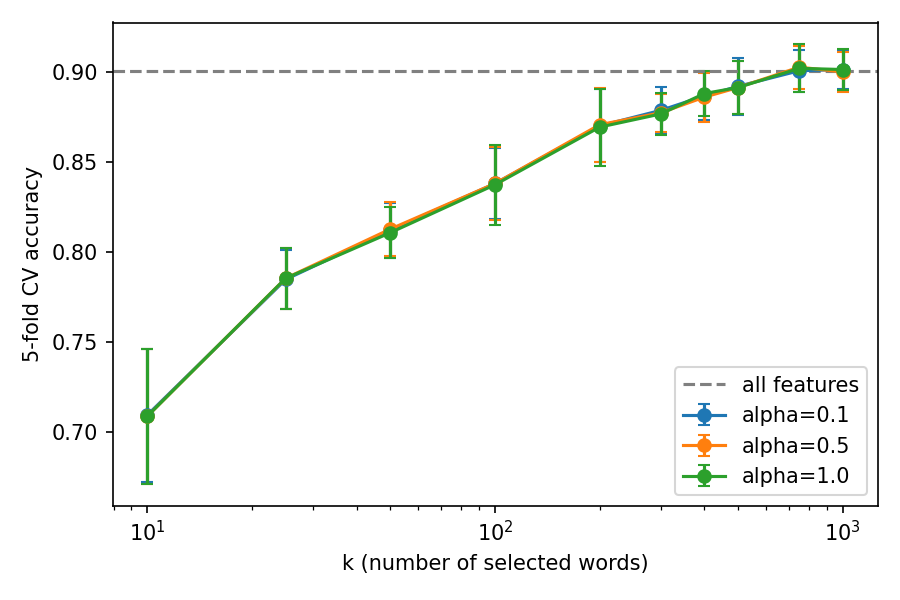
\includegraphics[width=0.49\textwidth]{results/figures/cv_nb.png}\hfill
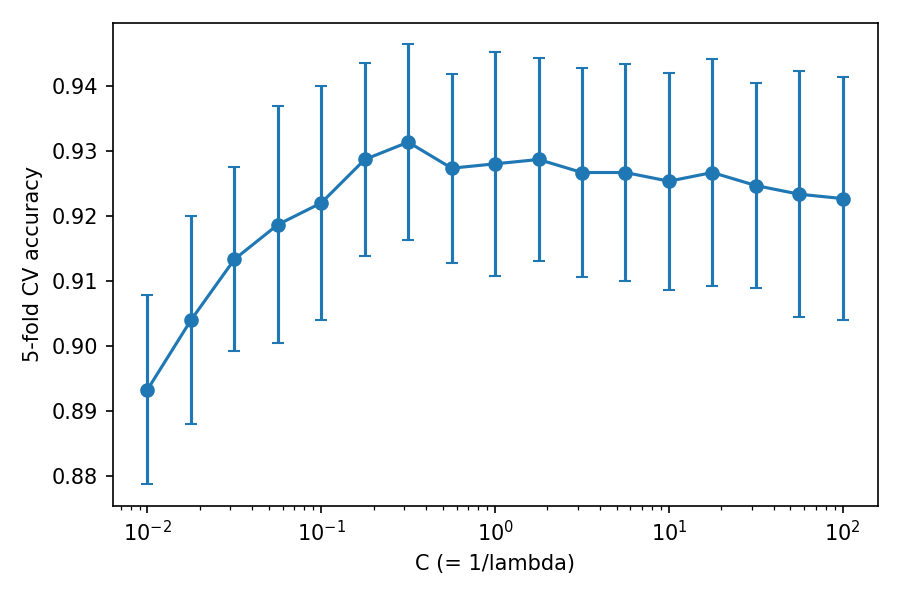
\includegraphics[width=0.49\textwidth]{results/figures/cv_lr.png}
\caption{Cross-validation accuracy of naive Bayes (left) and Lasso logistic regression (right).}
\label{fig:cv-linear}
\end{figure}

\begin{figure}[ht]
\centering
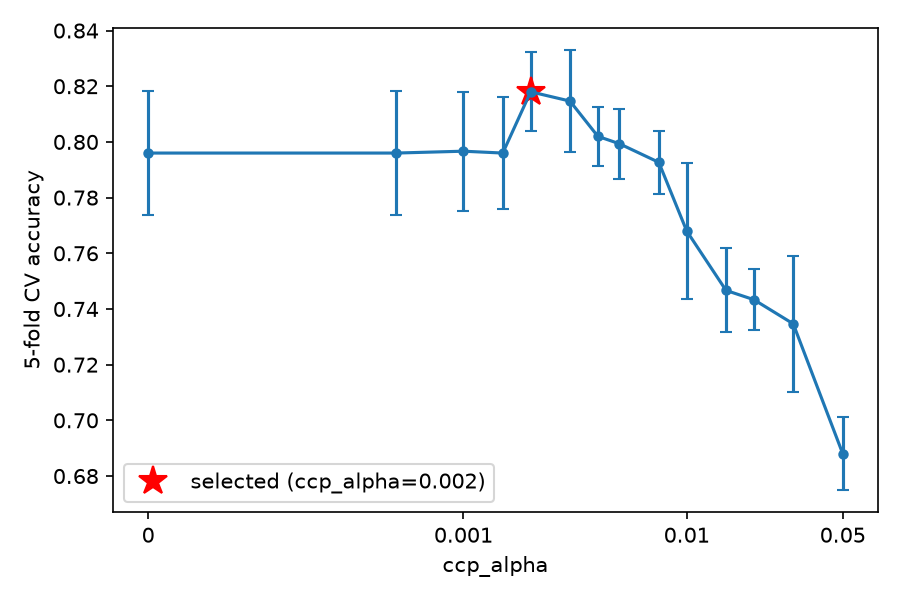
\includegraphics[width=0.49\textwidth]{results/figures/cv_tree.png}\hfill
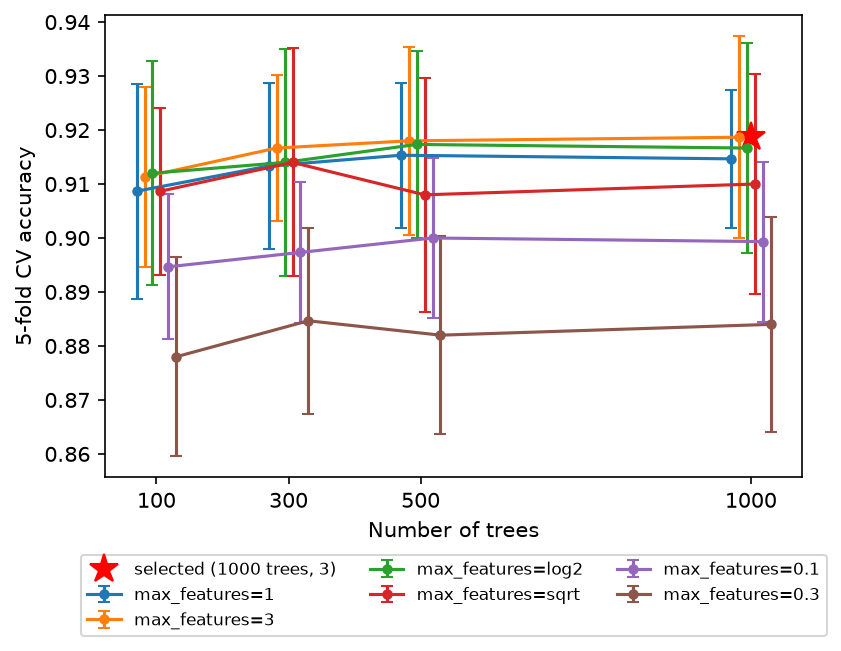
\includegraphics[width=0.49\textwidth]{results/figures/cv_rf.png}
\caption{Cross-validation accuracy of the classification tree (left) and random forest (right).}
\label{fig:cv-trees}
\end{figure}

\begin{figure}[ht]
\centering
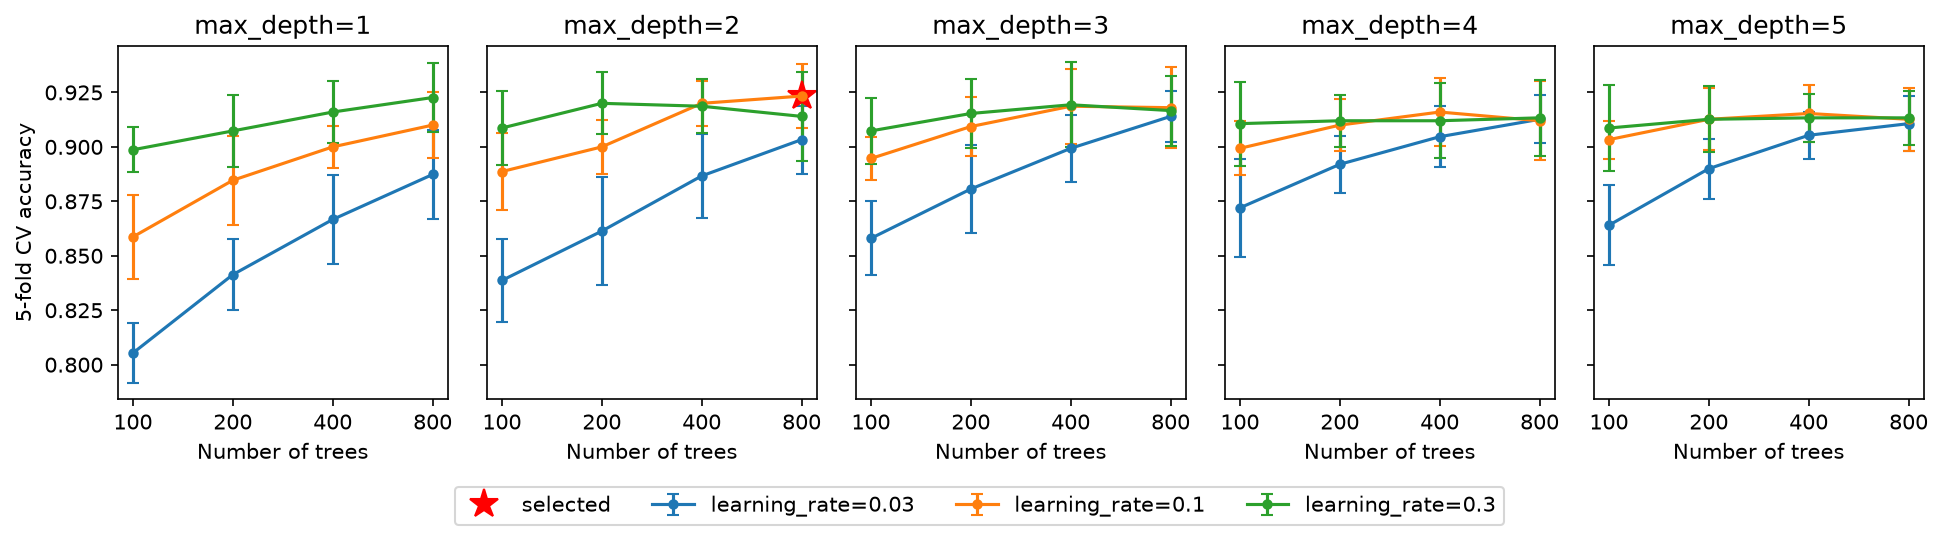
\includegraphics[width=\textwidth]{results/figures/cv_gb.png}
\caption{Cross-validation accuracy of gradient boosting, one panel per maximum tree depth.}
\label{fig:cv-gb}
\end{figure}

\section{Preprocessing comparison}
\label{app:prep}

Table~\ref{tab:prep} reports the comparison of preprocessing settings described in Section~3, produced by \texttt{src/compare\_preprocessing.py}. Accuracy is the mean over the same five training folds used for tuning, with the standard deviation in parentheses. Naive Bayes used $\alpha=1$ without feature selection. For Lasso logistic regression, $C$ was chosen from ten log-spaced values by an inner five-fold cross-validation within each training fold. Unless stated otherwise, every setting keeps stop words, uses no stemming, uses unigrams, and removes terms that occur in fewer than five training reviews.

\begin{table}[ht]
\centering
\caption{Five-fold cross-validation accuracy of naive Bayes and Lasso logistic regression under different preprocessing settings.}
\label{tab:prep}
\small
\begin{tabular}{@{}lrrr@{}}
\toprule
Setting & Terms & Naive Bayes & Lasso LR \\
\midrule
No sparse-term removal ($\mathrm{min\_df}=1$) & 4,737 & 0.894 (0.013) & 0.909 (0.022) \\
\textbf{Selected} ($\mathrm{min\_df}=5$) & 1,351 & 0.901 (0.010) & 0.899 (0.022) \\
$\mathrm{min\_df}=10$ & 845 & 0.895 (0.010) & 0.907 (0.019) \\
Stop words removed & 1,138 & 0.897 (0.016) & 0.893 (0.013) \\
Stemming & 1,186 & 0.895 (0.013) & 0.905 (0.020) \\
Stop words removed + stemming & 1,003 & 0.885 (0.013) & 0.901 (0.020) \\
Unigrams + bigrams & 3,665 & 0.908 (0.011) & 0.906 (0.022) \\
\bottomrule
\end{tabular}
\end{table}

\clearpage
\section*{AI disclosure statement}

We, Jiacheng Cai, Rongjian Gao, and Yanpeng Wang, confirm that the submitted work is our own work. Generative AI tools were used only as learning and writing aids for the activities summarized below. We checked the generated output and accept responsibility for the accuracy and validity of the submitted work.

\begin{table}[h!]
\centering
\small
\begin{tabular}{@{}p{1.8cm}p{9.0cm}p{2.5cm}@{}}
\toprule
Tool & Purpose & Used by \\
\midrule
ChatGPT & Summarizing  & Jiacheng Cai \\
\midrule
ChatGPT & Summarizing information, explaining concepts, and checking grammar. & Rongjian Gao \\
\midrule
OpenAI & To check the evaluation code. To draft the outlines of report. And to draw the tables in the reports. & Yanpeng Wang \\
\bottomrule
\end{tabular}
\caption{Overview of generative AI tools used.}
\label{tab:ai-tools}
\end{table}

\noindent Names of all students declaring that the statement above is accurate:\
Jiacheng Cai, Rongjian Gao, Yanpeng Wang\\
Date: \today



\end{document}
